\documentclass{standalone}
\usepackage{tikz}
\usepackage{graphicx}

\begin{document}

\begin{tikzpicture}[scale=0.75,transform shape]

\tikzset{
    nodeStyle/.style={circle, shift={(#1:0.3cm)}, draw=olive, inner sep=1pt}
}

% USE in Ausarbeitung
\node[anchor=south west, inner sep=0] (img) at (0,0)
{\includegraphics[width=10cm]{../graphics/Enveloppe/verlustbehaftet/R-1Abs}};

% USE stand-alone
%\node[anchor=south west, inner sep=0] (img) at (0,0)
%{\includegraphics[width=10cm]{../Enveloppe/verlustbehaftet/R-1Abs}};

%\draw[help lines] grid (10, 6);

% Position 1
\draw[fill=red, draw=red] (9.7,0.9) circle[radius=1pt] node[nodeStyle=0] {1};

% Position 2
\draw[fill=red, draw=red] (9.53,2.5) circle[radius=1pt] node[nodeStyle=0] {2};

% Position 3
\draw[fill=red, draw=red] (9.06,4.65) circle[radius=1pt] node[nodeStyle=90] {3};

% Position 4
\draw[fill=red, draw=red] (8.4,1.39) circle[radius=1pt] node[nodeStyle=-90] {4};

% Position 5
\draw[fill=red, draw=red] (7.75,4.73) circle[radius=1pt] node[nodeStyle=90] {5};


\draw (4.5, 5.17) -- (5.25,5.5) node[right] {$|U_{h}| + |U_{r}|$};
\draw (4, 3.15) -- (3.75,2.5) node[below] {$|U_{h}| - |U_{r}|$};

\end{tikzpicture}

\end{document}